%% Based on a TeXnicCenter-Template by Tino Weinkauf.
%%%%%%%%%%%%%%%%%%%%%%%%%%%%%%%%%%%%%%%%%%%%%%%%%%%%%%%%%%%%%

%% TODO
%%   fix fonts - which font; do headings also change?
%%   fix Tex path to find fonts; pick a font
%%   printed vs. displayed hyperlinks
%%   hypersetup customization?
%%   widen margins - DONE
%%   use oneside or twoside? 10, 11 12pt ?

%%%%%%%%%%%%%%%%%%%%%%%%%%%%%%%%%%%%%%%%%%%%%%%%%%%%%%%%%%%%%
%% HEADER
%%%%%%%%%%%%%%%%%%%%%%%%%%%%%%%%%%%%%%%%%%%%%%%%%%%%%%%%%%%%%

%%\documentclass[12pt,oneside]{report}
\documentclass{llncs}

%% Language %%%%%%%%%%%%%%%%%%%%%%%%%%%%%%%%%%%%%%%%%%%%%%%%%
%\usepackage[USenglish]{babel} %francais, polish, spanish, ...
%\usepackage[T1]{fontenc}
%\usepackage{textcomp}
%\usepackage[ansinew]{inputenc}
%\usepackage{makeidx}	  %% needed to create an index
\usepackage{hyperref}   %% sets hyperlinks within a pdf
\usepackage{graphicx}
\usepackage{epstopdf}
\usepackage{parskip}
\usepackage{subcaption}

%%\usepackage{lmodern} %Type1-font for non-english texts and characters


%% Packages for Graphics & Figures %%%%%%%%%%%%%%%%%%%%%%%%%%
%\usepackage{graphicx} %%For loading graphic files
%\usepackage{subfig} %%Subfigures inside a figure
%\usepackage{tikz} %%Generate vector graphics from within LaTeX

%\usepackage{mathptmx} %% Times fonts, for math as well


%%\makeindex

%% The adjustment amounts depend on the font
%% -.5 for 12pt, -.875 for 10pt
%% FIXME: should these be set instead of adjusted?
\addtolength{\oddsidemargin}{-.5in}
\addtolength{\evensidemargin}{-.5in}
\addtolength{\textwidth}{1.0in}
\addtolength{\topmargin}{-.5in}
\addtolength{\textheight}{1.0in}

\newcommand{\tjark}[1]{\marginpar{\footnotesize{#1}}}
\newcommand{\tjarkx}[1]{\makebox[0pt][c]{\raisebox{0pt}[0pt][0pt]{\Large\textcolor{red}{${}^*$}}}\marginpar{\footnotesize{#1}}}


\begin{document}


\title{The 2014 SMT Competition}

\author{David R. Cok (chair of organizing committee)\inst{1} \and \\ 
David DeHarbe (co-organizer)\inst{2} \and \\ 
Tjark Weber (co-organizer)\inst{3} 
}

\institute{GrammaTech, Inc.,  \email{dcok@grammatech.com} \\
\and
Federal University of Rio Grande do Norte, Brazil \email{David.Deharbe@loria.fr} \\
\and
Uppsala University, Sweden \email{tjark.weber@it.uu.se} 
}

\maketitle
\pagestyle{plain}
\pagenumbering{arabic}

\abstract{The 2014 SMT Competition was held in conjunction with the SMT workshop, affiliated with the CAV, IJCAR, and SAT conferences at FLoC 2014\cite{TBD}, at the Vienna Summer of Logic\cite{TBD} in July 2014. Eighteen solvers participated from fourteen different research groups, across 34 different logic divisions. The competition was also part of the FLoC Olympic Games event, which gave combined visibility to 14 different competitions related to automated logic problem solving.} 
\tjarkx{A couple sentences on notable innovations or results}


\section{Introduction}
The 2014 SMT Competition continued the series of annual competitions in SMT solver capability and performance that began in 2005. This is the 9th competition in the series, skipping only 2013; in that year an evaluation \cite{TBD} was performed, rather than a competition.

The competition is held to spur advances in
SMT solver implementations acting on benchmark formulas of practical interest. Public competitions are
a well-known means of stimulating advancement in software tools. For example, in automated
reasoning, the SAT and CASC competitions for propositional and first-order reasoning tools, respectively,
have spurred significant innovation in their fields \cite{leberre+03,PSS02}.

The competition is sponsored by the SMT workshop, which was hled in conjunction with the
CAV, IJCAR, and SAT conferences at FLoC 2014\cite{TBD}, at the Vienna Summer of Logic\cite{TBD} in July 2014.
Information about the winners
and results of the competition is summarized in this report and is available online at \url{www.smtcomp.org}; information
about previous years' competitions is also available at that website and in a published summary reports \cite{springerlink:10.1007/s10817-012-9246-5}.\tjark{Cite 2012 and 2013 as well}

\section{Context of the competition}

The SMT Competition is a competition among SMT solvers on a set of benchmark logic problems expressed in the SMT-LIB \cite{TBD} language. Each benchmark problem is a combination of definitions and logical assertions expressed with respect to an underlying logical theory and, perhaps, some constraints on the kinds of expressions in that theory. Each problem has a set of constant or function symbols; a solution to the problem is an assignment of each constant and function evalution to logical values in a way that satisfies all the problem's assertions. That is, the problem is to find a \textit{satisfying assignment} for the benchmark problem. For example, a problem might be simply a set of assertions in 
propositional logic, in terms of Boolean constants such as $P$, $Q$, and $R$.

As stated, the goal is the same as the SAT competition. The SMT benchmarks extend SAT by incorporating defined theories, such as the theory of arrays, or of undefined functions, or of arithmetic, or of bit-vectors. In addition, there may be constraints on the set of expressions allowed, such as only linear arithmetic, or only integer difference arithmetic. The theories also define \textit{sorts}, which make the theories a kind of typed first-order logic. Examples of sorts used in current theories are Boolean, Int, Real, bit-vectors of various lengths, and arrays with arbitrary sorts as index and value. Each combination of underlying theories and language constraints is a \textit{logic}.

The benchmark problems are expressed in the concrete syntax defined in the SMT-LIB (v2) standard \cite{TBD}. This standard has been used since 2010, and a previous version was used prior to that. One of the goals of the SMT competition is to encourage use and tool implementations of the SMT-LIB standard.
\tjark{Give an example of a benchmark in SMT-LIB} \tjark{Provide information about the sizes of benchmarks}

SMT (Satisfiability Modulo Theories) solvers are automated tools that seek to find a satisfying assignment for a given SMT-LIB problem, or to assure that the problem is \textit{unsatisfiable}.
Tools may not be able to solve a given problem, because, for example the tool exhausts available memory or time; a tool is permitted to answer \textit{unknown}. However, giving an incorrect answer (\textit{sat} instead of \textit{unsat}, or vice versa) is considered \textit{unsound} and a serious fault in the tool.

SMT differs from the CASC competition \cite{TBD} in directly addressing sorted logics. SMT also focuses on fragments of first-order logic that are \textit{decidable}. For example, a subset of the benchmarks are problems in an integer-difference logic, for which there are specific decision procedures. The competition among tools is to create very efficient implementations of a breadth of decision procedures. Accordingly, SMT solvers have historically also not handled logics with quantified expressions, though several currently now do so.

\section{The Competition Goals and Organization}

In planning the 2014 competition, the organizers' overall goal was to encourage breadth
in the capability of SMT solvers. SMTCOMP 2014 benefited from the evaulation that was performed in 2013 and the experience of the 2012 competition. As a result we established the following emphases:
\begin{itemize}
\item In 2012 we narrowed the competition to a smaller number of more significant logics. In response to feedback, in 2014 we reverted to the practice of evaluating solvers in all available divisions.


\end{itemize}

Previous years have challenged solvers to support a variety of logics and
have measured them on raw performance on individual problems. This year we have two additional goals. First, we
focused the competition on a subset of the logics that are the more relevant to applications. Some of the 
simpler logics are now routine for nearly all solvers and therefore not a good basis for a competition. Others have 
received only light interest in the past. Some of the less expressive logics are subsumed into the more expressive logics
for selecting competition benchmarks.

Second, we
wished to encourage support for additional capabilities, namely, determining unsatisfiable cores and generating proofs.
Finding small unsatisfiable cores is important, for example, in finding contradictions within sets of assertions; compact unsatisfiable cores also produce more compact proofs. Finding a {\em minimal} unsatisfiable core is a hard problem with no known practical algorithm;
thus, good heuristics that apply to problems of interest are valuable and worth a competition. So, the organizers added
an unsat core track to the 2012 competition. The winner of that track is the solver that, without producing any erroneous results, produces the smallest unsatisfiable cores on the benchmark set within the timeout period.

Similarly, constructing proofs of unsatisfiability is also useful, particularly if quantified assertions are included.
Since there is as yet no standard method to express proofs and thus no easy way to check them, the organizers added a proof generation track solely in demonstration mode. We encouraged submission of solvers with this capability, but we did not attempt to measure the speed or accuracy of such solvers this year. We do hope that
attention to proof generation will encourage standardization of proof format and of proof checkers.

The competition used a subset of benchmarks from those available at \url{www.smtlib.org}. The full benchmark suite contains about 100,000 benchmarks. New benchmarks are continually being added --- additional benchmarks were added to the main and application tracks for 2012. The unsat core benchmarks were adapted from main track benchmarks that are unsatisfiable. The benchmarks are a collection of more or less relevant problems, rather than benchmarks that measure specific metrics.
Some benchmarks are families of constructed problems of arbitrary size; these can test the scalability of a solver as
the size of the benchmark instance is increased. Other benchmarks are formed from problems that arise in actual 
applications. For example, software verification of real programs produces many SMT problems that are suitable as benchmarks.

The full description of the 2012 SMT competition's rules is found in the rules document (\url{www.smtcomp.org/2012/rules12.pdf}). The document describes the procedures for determining benchmark difficulties, selecting benchmarks for competition, and judging the results.

\paragraph{Procedure.} 

The competition's traditional `main' track tests a solver's ability to determine the satisfiability or unsatisfiability of a single problem (perhaps with multiple assertions) within a given logic. A second track tests the performance of multi-threaded solvers on similar problems.

The `application' or incremental track, introduced last year, tests a qualitatively different capability. Software verification tools often use SMT solvers as a back-end proof engine. These tools repeatedly invoke the solver with different, related satisfiability problems; the problems may have a substantially similar set of assertions, produced by the tool's adjusting, correcting, adding, or retracting assertions interactively; in batch mode different properties may be checked using substantially the same set of assertions.
The effect is that the solver must respond to a sequence of requests to assert or retract logical statements, check satisfiability, produce counterexamples, and so on. The application track tests a solver's performance in responding to such a sequence of commands, as produced by actual application problems. To implement the application track benchmarks, the 
competition uses a simulation engine that communicates with the solver just like an application (or a user at a keyboard) would, presenting each command and waiting for a response before presenting the next command; this mechanism (appropriately) prevents a solver from optimizing its effort based on knowing the entire sequence of commands all at once. A report
on the first (2011) year's application track and the overall design was presented by Griggio and Bruttomesso at the 
2012 COMPARE Workshop \cite{ag+rb+12}.

The benchmarks are each assigned a {\em difficulty}. The difficulty is based on how long it takes a group of solvers to produce a correct answer to the benchmark. For competition, benchmarks are selected, at random, from each difficulty category. 

The winning solver in each category is the one that produces the most correct answers in the least time. An additional change this year is that incorrect answers are a disqualifier: the organizers considered that solver technology has progressed sufficiently in capability and importance that incorrect answers should not be tolerated (a solver can always intentionally produce an answer of `unknown'). Each solver is given a fixed timeout period (this year the timeout was 20 minutes) in which to answer a benchmark. The winner is the solver that produces the most correct (non-{\em unknown}) answers and no incorrect answers; in the case of ties, the winner is the solver that took the least time to produce its correct answers.\footnote{There is an anomaly in this scoring system. Solvers A and B may produce the same correct answers, with A taking slightly less time to do so than B, and thus being the winner. Answers of {\em unknown} do not count towards correct answers, but the time taken also does not penalize the total time used. It may be the case the A takes a long time to determine an answer of {\em unknown} on some benchmarks, where as B can do so quickly. Thus B may be overall preferable in an application, even though A is the competition winner.}
In the unsat-core track, it is the size reduction of the core that is measured, rather than the number of correct answers.

\paragraph{The competition infrastructure.} The competition is executed on a cluster of machines at the University of Iowa, under the control of the SMT-EXEC software suite (cf. \url{www.smtexec.org}). This software suite has been used in past years as well. A new hardware and software infrastructure, Star-Exec (cf. \url{www.starexec.org}), is under development and was the subject of the Star-Exec workshop at IJCAR'12.

\paragraph{The SMTLIB language.} A competition based on benchmark problems needs a standard language in which to express those problems.
For SMTCOMP, that language is the SMT-LIB language (cf. \url{www.smtlib.org}, \cite{BarST-SMT-10} \cite{Cok-SMTLIBTutorial-2011}). 
In 2010, a significantly reworked version of the language was agreed upon.
This version 2 increased the flexibility and expressiveness of the language while also simplifying the syntax. 
It also includes a command language that improves the language's usefulness for interactive applications.
In particular, the standard specifies a typed (sorted), first-order logical language for terms and formulas, a language for specifying background logical theories and logics, and the command language. Some other tools that process SMT-LIBv2 are listed in the SMT-LIB web pages (cf. \url{http://www.smtlib.org/utilities.html}).

\section{Participants}

\paragraph{Solvers.} The competition registration includes information about each competing solver. In addition, some solver groups provided summaries of their solvers and their recent technical advances. The provided summaries are included in these proceedings as additional papers. Note that although one person is listed as the `submitter', there is generally a team of contributors behind each tool. The 2012 participants were the following:
\begin{itemize}
\item 4Simp - submitted by Trevor Hansen, U. Melbourne
\item AbzizPortfolio - submitted by Mohammed Adbul Aziz, U. Cairo. (This solver is unusual in that it is a portfolio solver: based on automated learning over benchmark characteristics, it chooses among 5 other solvers from the 2011 competition to apply to the problem at hand.)
\item Boolector - submitted by Armin Biere, Johnnes Kepler University
\item CVC3 v2.4.2 - submitted by Morgan Deters, NYU
\item CVC4 1.0rc.3931 - submitted by the ACSys Group, NYU
\item MathSAT-HeavyBV - submitted by Bas Schaafsma, U. Trento and FBK
\item MathSAT5-smtcomp12 - submitted by Alberto Griggio, U. Trento and FBK (with variations submitted to the application and unsat core tracks)
\item SMTInterpol - submitted by Jochen Hoenicke, U. Freiburg
\item SONOLAR - submitted by Florian Lapschies, U. Bremen
\item STP2 - submitted by Trevor Hansen, U. Melbourne, and Vijay Ganesh, MIT
\item Tiffany de Wintermonte \& Sonolar - submitted by Trevor Hansen, U. Melbourne
\end{itemize}

\begin{table}[t]
\centering
\begin{tabular}{|l|l|c|c|c|c|c|c|c|c|}
\hline
Solver & Affiliation & 2005 & 2006 & 2007 & 2008 & 2009 & 2010 & 2011 & 2012 \\
\hline
4Simp	                 & U. Melbourne   &   &   &   &   &   &   &   & X \\								
Tiffany de Wintermonte & U. Melbourne 	&   &   &   &   &   &   &   & X \\							
AbzizPortfolio         & U. Cairo       &   &   &   &   &   &   &   & X \\							
Boolector              & J.K. U.        &   &   &   & X & X &   & X & X \\
CVC/CVCLite/CVC3       & NYU, U. Iowa   & X & X & X & X & X & X & X & X \\
CVC4	                 & NYU, U. Iowa   &   &   &   &   &   & X & X & X \\
MathSat-HeavyBV        & U. Trento      &   &   &   &   &   &   &   & X \\								
MathSAT 3,4,5          & U. Trento, FBK & X & X & X & X & X & X & X & X \\
SMTInterpol            & U. Freiburg    &   &   &   &   &   &   & X & X \\
SONOLAR                & U. Bremen      &   &   &   &   &   & X & X & X \\
STP, STP2              & MIT            &   & X &   &   & X &   & X & X \\
AProVE NIA             & RWTH Aachen    &   &   &   &   &   & X & X &   \\
opensmt                & U. Lugano      &   &   &   & X & X & X & X &   \\
veriT                  & UFRN           &   &   &   &   & X & X & X &   \\
Z3                & Microsoft Research  &   &   & X & X &   &   & X &   \\
MiniSMT                & U. Innsbruck   &   &   &   &   &   & X &   &   \\	
simplifyingSTP         & U. Melbourne   &   &   &   &   &   & X &   &   \\	
test\_pmathsat         & FBK-IRST       &   &   &   &   &   & X &   &   \\	
barcelogic             & UPC            & X & X & X & X & X &   &   &   \\	
beaver                 & UC BVerkeley   &   &   &   & X & X &   &   &   \\		
clsat                  & Washington U.  &   &   &   & X & X &   &   &   \\		
Sateen                 & U. Col-Boulder & X & X & X & X & X &   &   &   \\		
sword                  & U. Bremen      &   &   &   & X & X &   &   &   \\		
Yices                  & SRI            & X & X & X & X & X &   &   &   \\		
Spear                  &   &   &   & X & X &   &   &   &   \\		
Alt-Ergo               &   &   &   &   & X &   &   &   &   \\			
ArgoLib                &   &   &   & X &   &   &   &   &   \\				
Fx7                    &   &   &   & X &   &   &   &   &   \\				
Ario                   &   & X & X &   &   &   &   &   &   \\					
ExtSat                 &   &   & X &   &   &   &   &   &   \\					
HTP                    &   & X & X &   &   &   &   &   &   \\					
Jat                    &   &   & X &   &   &   &   &   &   \\					
NuSMV                  &   &   & X &   &   &   &   &   &   \\					
Sammy                  &   & X &   &   &   &   &   &   &   \\						
SBT                    &   & X &   &   &   &   &   &   &   \\						
Simplics               &   & X &   &   &   &   &   &   &   \\					
SVC	                   &   & X &   &   &   &   &   &   &   \\	
\hline					
\end{tabular}
\vspace{.2in}
\caption{History of solver participation}
\label{Table:participants}
\end{table}

\begin{table}
\centering
\begin{tabular}{|l|c|c|c|c|c|c|c|c|}
\hline
 & 2005 & 2006 & 2007 & 2008 & 2009 & 2010 & 2011 & 2012 \\
\hline
Participants                 & 12 & 12 & 9 & 13 & 12 & 10 & 11 & 11 \\
New in given year            & 12 &  4 & 4 &  6 &  2 &  6 &  1 &  4 \\
Continuing to the next year  &  8 &  6 & 7 & 10 &  4 &  7 &  7 &    \\
Not ever participating again &  4 &  5 & 2 &  2 &  6 &  3 &  4 &    \\ 
\hline
\end{tabular}
\vspace{.2in}
\caption{Changes in participation}
\label{Table:changes}
\end{table}

\paragraph{History.} The number of solvers competing each year has consistently remained in the range of 9-13 entrants.
Some solvers have competed for several consecutive years. Others are new entrants. The introduction in 2010 of SMT-LIBv2 as the standard language for benchmarks was a significant event. The new language required solvers to revise their front-ends and to add new capabilities.
As a result, some solvers did not continue participating, at least not immediately. However, the use of SMTLIBv2 also increased the expressiveness of benchmarks. Thus benchmarks representing the needs of industrial applications were able to be added; 
the application track of the competition was added to demonstrate this capability and the corresponding abilities of solvers.


Table \ref{Table:participants} shows the history of participation in SMTCOMP, with Table \ref{Table:changes} summarizing some statistics. The number of solvers in 2012 is typical of past years. Note though that within the fairly stable total number there has been a punctuated evolution in the actual participants. The competitions in 2009 and 2011 had only a few new participants, but otherwise roughly a third of the participants each year are new, and these are not just new solvers from existing groups, but include new participating researchers as well. A few solvers have been very long-term participants, particularly CVC and MathSAT. The largest single year change was from 2009-2010: half the 2009 solvers did not participate again and this transition saw the lowest number of continuing participants, presumably due to the change in benchmark format.

\section{Results}

\paragraph{New benchmarks.} One of the goals of the SMT competition is to accumulate benchmark problems. These are, of course, used in the competition. But they are also useful as part of the overall SMT endeavor. Researchers can use the SMT benchmarks for studies of benchmark characteristics, solver evaluation, and their own solver testing quite apart from any competition. In particular, it is important to accumulate increasing numbers of benchmarks relevant to actual application areas. More benchmarks are needed that reflect software verification problems, but other constraint satisfaction domains, such as planning and optimization, are also needed.

Benchmark submissions come from the SMT community; the organizers check the benchmarks and prepare them for competition and for the SMT benchmark library.
SMT-LIB currently has about 100,000 benchmarks. An additional 13,811 main track benchmarks were submitted in 2012 (though they were not ready in time to be used in the competition). They fell into these categories:
\begin{itemize}
\item Main track benchmarks were added in these divisions (cf. \url{http://smtexec.org/2012_benchmarks/main/list.txt}):
\begin{itemize}
\item AUFNIRA: 190
\item NIA: 26
\item NRA: 21
\item QF\_AUFBV: 39
\item QF\_IDL: 30
\item QF\_LIA: 513
\item QF\_NRA: 12949
\item UFNIA: 39
\item UFRIA: 4
\end{itemize}
As the list above shows, a large number of QF\_NRA benchmarks were added, but only small numbers in other divisions.
\item The application track has about 1056 benchmarks from 2011. In 2012 we added about 150.
\item Unsat core benchmarks were derived from selected main track benchmarks by adding the command to generate unsat cores. The competition benchmarks were selected from these divisions
\begin{itemize}
\item 2584 QF\_LIA benchmarks
\item  317 QF\_LRA benchmarks
\item  683 QF\_IDL benchmarks
\item 1399 QF\_BV benchmarks
\end{itemize}
\end{itemize}

\paragraph{Main track.} The organizers invited submissions to 8 competitive divisions in the main track; of those, 4 had sufficient participation to be competitive. Note that the previous year's winners are automatically included for comparison but are not counted in the `participants' and are not eligible to be declared the winner for the year:
\begin{itemize}
\item QF\_BV: 9 participants; Winner: Boolector; Open-source winner: Boolector; improved over 2011 winner (Z3)
\item QF\_AUFBV: 6 participants; Winner: Boolector; Open-source winner: Boolector; improved over 2011 winner (Boolector)
\item QF\_UFLIA: 4 participants; Winner: MathSAT5; Open-source winner: SMTInterpol; not improved over 2011 (Z3)
\footnote{CVC4 scored lower than the others because a rare bug caused an incorrect result on one benchmark, and any solver with errors scores lower than those without; the patched resubmission would have placed second and would have been the open-source winner.}
\item QF\_UFLRA: 4 participants; Winner: CVC4; Open-source winner: CVC4; improved over one but not the other of the co-winners in 2011.
\end{itemize}

Four additional divisions (QF\_IDL, AUFLIA+p, AUFLIA-p, and AUFNIRA) had only two submissions (CVC3 and CVC4) and so were run only as demonstrations. These did not improve over the 2011 winner (Z3).

In addition, any other division was run as a demonstration, if there were submissions in that division. Since these were advertised only as demonstration runs, the participants did not necessarily optimize or test their solvers for these divisions. Thus conclusions should not be drawn from their performance. These divisions were
\begin{itemize}
\item QF\_UF: 4 participants
\item QF\_AUFLIA: 3 participants
\item QF\_LRA: 4 participants
\item QF\_LIA: 4 participants
\end{itemize}
In each case, the 2011 winner (Z3) still out-performed the 2012 participants.

\paragraph{Application track.}

The application track had participation from just two solvers, MathSAT and SMTInterpol, in three divisions (QF\_UFLIA, QF\_LRA, and QF\_LIA). These were also the participants last year, along with Z3 and, in one division, opensmt. The years are sufficiently different that no year-to-year comparisions can be made: there were many new benchmarks, and more benchmarks were run in 2012. 

\paragraph{Parallel track.} The competition invited submissions for a parallel track in 2012. No solvers were submitted to this track for 2012.  Parallel solvers were submitted in 2010 and 2011, but never enough to be competitive.

\paragraph{Unsat core track.} Two solvers (MathSAT and SMTInterpol) participated in the unsat-core demonstration track, in three divisions (QF\_LRA, QF\_LIA, and, with just MathSAT, QF\_BV). Generally speaking, the times taken for these benchmarks were quite small, with only a few timeouts. The key measure of success was the reduction in the number of assertions that constituted the unsatisfiable core - that is, the score is the difference between the total number of assertions in the benchmark and the number reported as the core. The reported cores were checked in an off-line step to be sure that they were still unsatisfiable, by the best three solvers of the 2011 competition for
the corresponding category.

\begin{figure}[t]
\centering
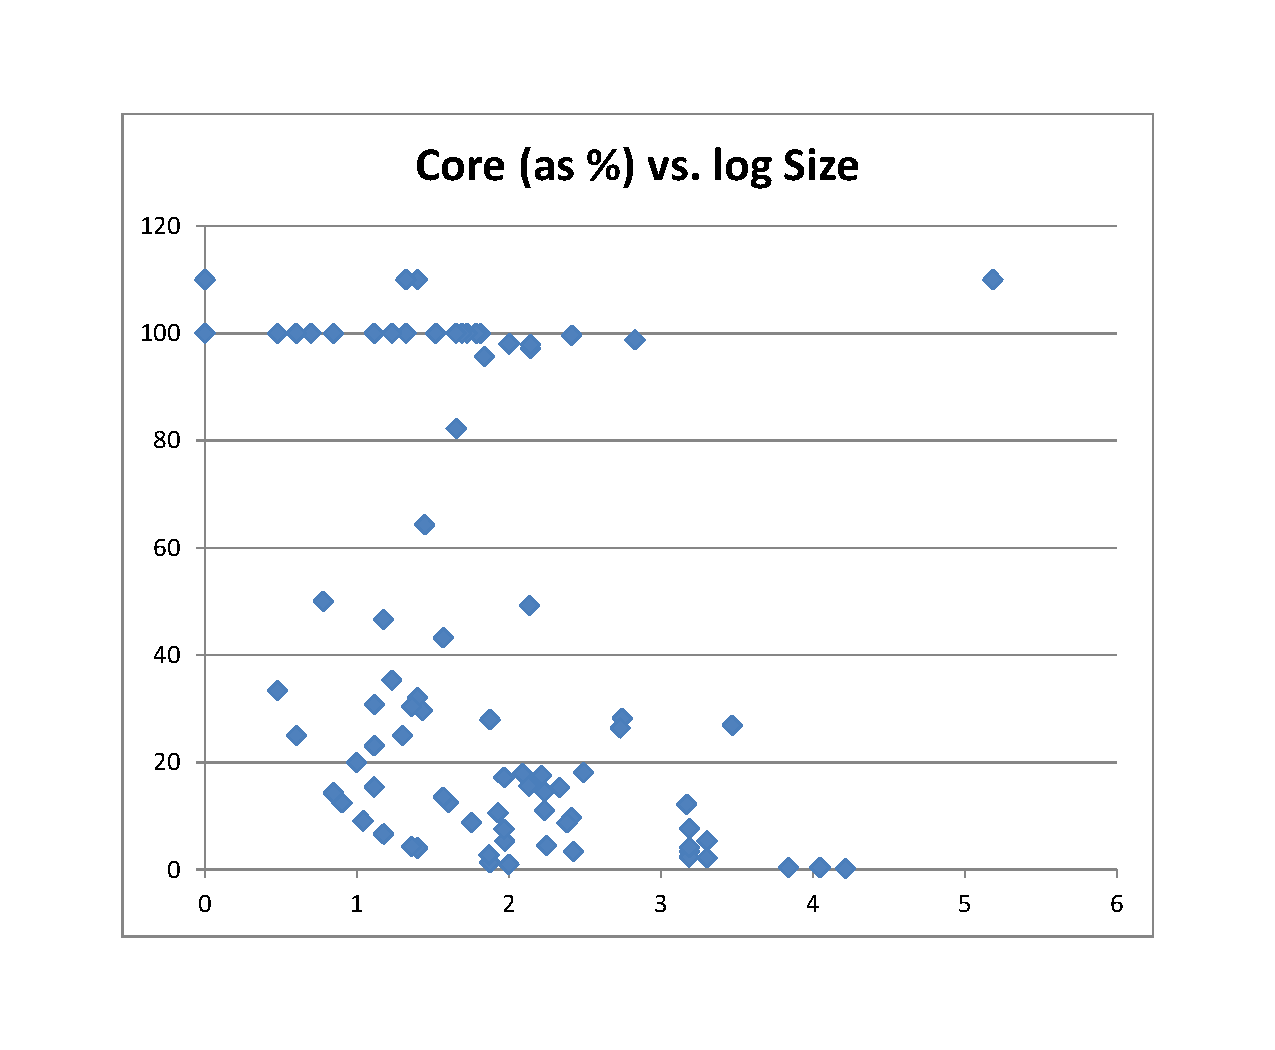
\includegraphics[width=\textwidth]{SMTCOMP-Core2.pdf}
\caption{Sizes of unsat cores as fraction of original, vs. $log_{10}$ of the number of assertions in the benchmark. Timeouts are shown at 110\%.}
\label{Fig:cores}
\end{figure}

Figure \ref{Fig:cores} shows the size of the resulting unsatisfiable core as a fraction of the original number of assertions in the benchmark. Timeouts are shown on the graph as having a result size of 110\%, though in practice they would be 100\%, not having been successful at reducing the size of the unsat core. The horizontal axis is the log of the number of assertions in the benchmark, ranging from just a few to over 100,000. A fair number of the benchmarks show no or almost no reduction at all (the marks on or near the 100\% line). It is not known whether no reduction is possible or whether any reduction is too difficult for these solvers. The others range from 20\% reduction to over 90\% reduction.

\paragraph{Proof generation track.} There was just one submission in the proof-generation demonstration track, SMTInterpol. Thus we used this solver as an example of proof output. The organizers would like to encourage proof generation by SMT solvers, but there are some barriers to be surmounted before any competition is possible. The key need is for a standard way of expressing proofs, so that tools can be built to check them (as part of a competition). The difficulty is that solvers work in signficantly different ways, and thus their atomic proof steps may be quite different. A workshop at IJCAR 2012, Proof Exchange for Theorem Proving (PxTP), was held to discuss just this issue.

The system description for SMTInterpol included in the SMTCOMP'12 proceedings includes an outline of its proof format. A general overview of proof formats indicates that proofs will always be long and will be difficult for humans to read or check, and that creating a solver-independent format will be a challenge.

\section{Conclusions and future plans}

\paragraph{Measuring improvement.}


\begin{figure}[ht]
\centering
\begin{subfigure}{0.45\textwidth}
	   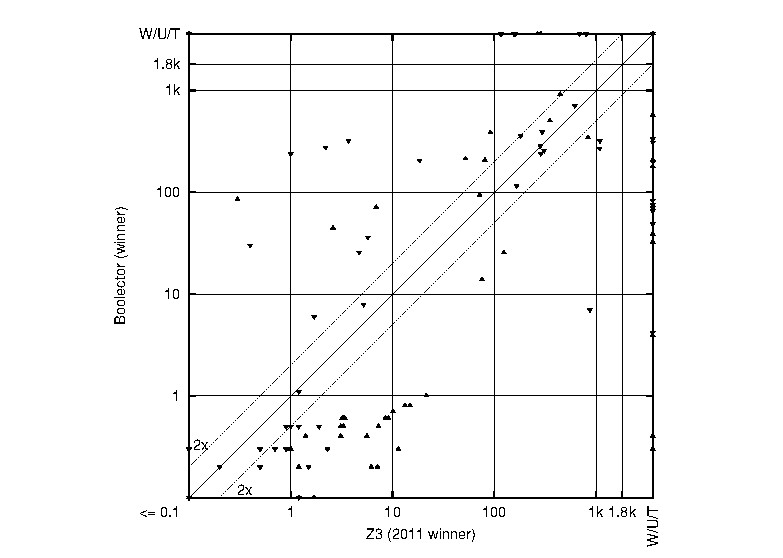
\includegraphics[width=1\textwidth]{QF_BV-scatter-improvement.eps}
	   \caption{QF\_BV benchmarks}
	\end{subfigure}
\begin{subfigure}{0.45\textwidth}
	   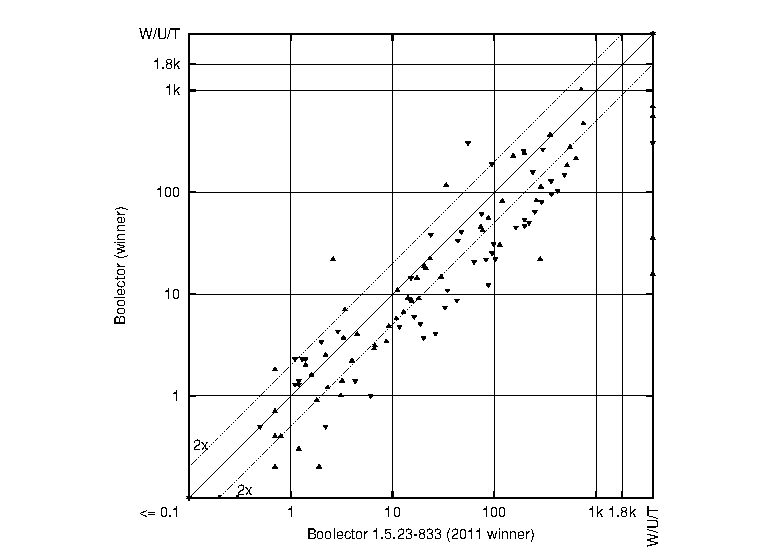
\includegraphics[width=1\textwidth]{QF_AUFBV-scatter-improvement.eps}
	   \caption{QF\_AUFBV benchmarks}
	\end{subfigure}
\begin{subfigure}{0.45\textwidth}
	   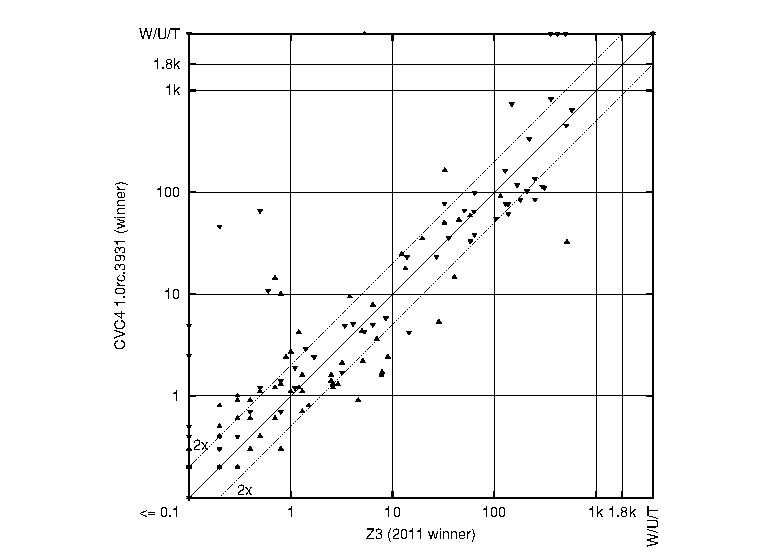
\includegraphics[width=1\textwidth]{QF_UFLRA-scatter-improvement.eps}
	   \caption{QF\_UFLRA benchmarks}
	\end{subfigure}
\begin{subfigure}{0.45\textwidth}
	   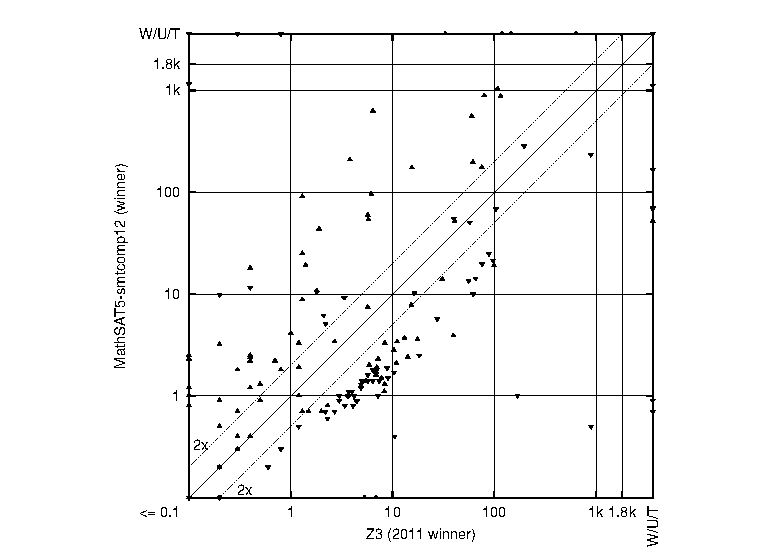
\includegraphics[width=1\textwidth]{QF_UFLIA-scatter-improvement.eps}
	   \caption{QF\_UFLIA benchmarks}
	\end{subfigure}	
\begin{subfigure}{0.45\textwidth}
	   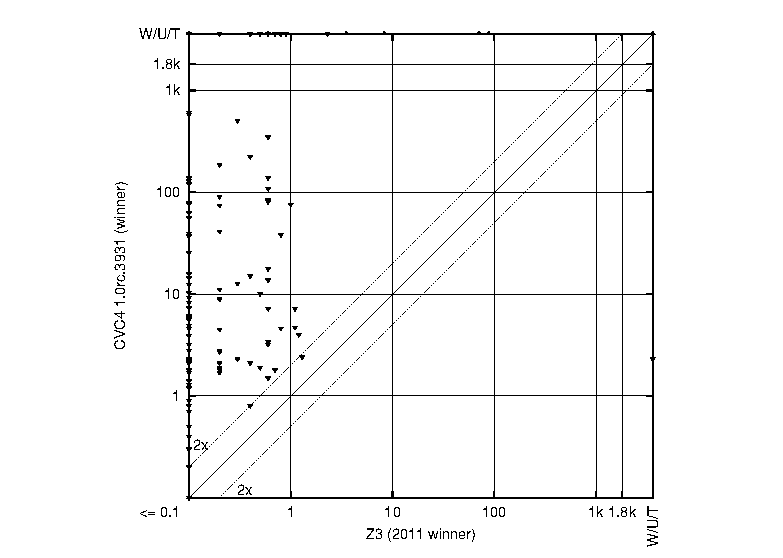
\includegraphics[width=1\textwidth]{AUFLIA+p-scatter-improvement.eps}
	   \caption{AUFLIA+p benchmarks}
	\end{subfigure}	
\begin{subfigure}{0.45\textwidth}
	   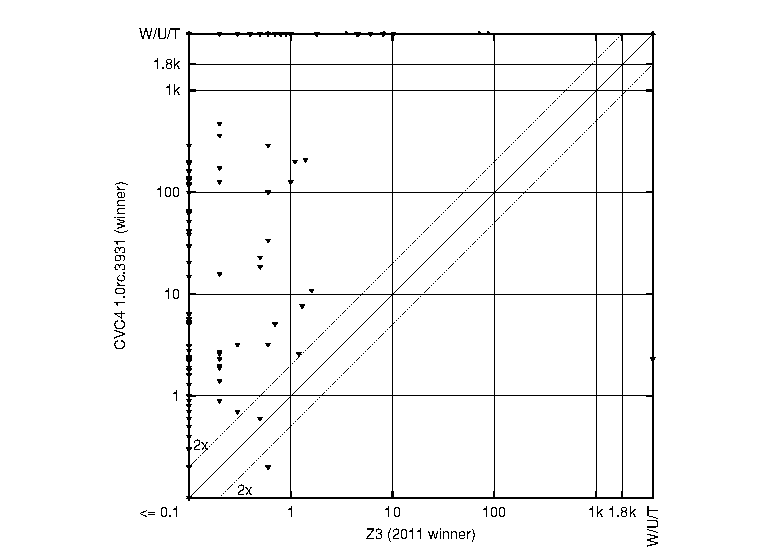
\includegraphics[width=1\textwidth]{AUFLIA-p-scatter-improvement.eps}
	   \caption{AUFLIA-p benchmarks}
	\end{subfigure}	
\begin{subfigure}{0.45\textwidth}
	   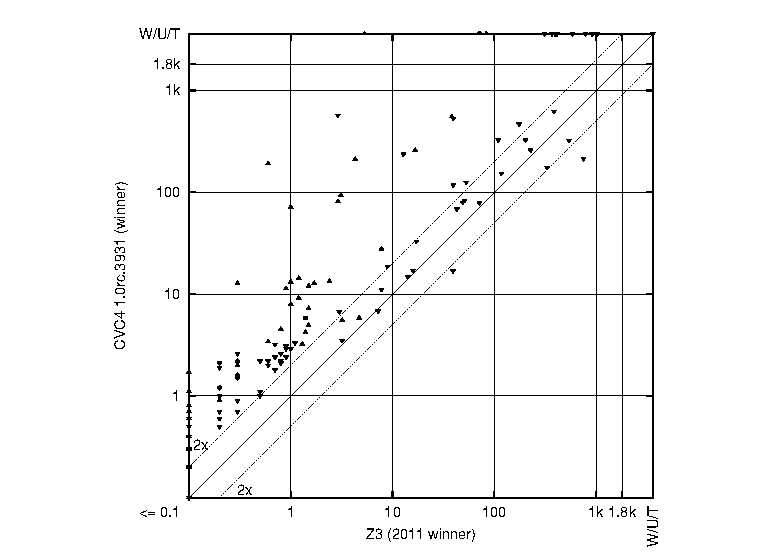
\includegraphics[width=1\textwidth]{QF_IDL-scatter-improvement.eps}
	   \caption{QF\_IDL benchmarks}
	\end{subfigure}	
\caption{Comparisons of 2012 and 2011 winners the main track divisions. The axes show time taken, so marks below and to the right of the diagonals show improvement in 2012.}
\label{Comparisons}
\end{figure}

One of the goals of a repeated competition is to prod improvement from year to year. Hence one would like measures of such improvement. We currently measure such improvement only in a limited sense in that we only make year-to-year comparisons on selected benchmarks. Such measures are imperfect because the set of solvers, the competition benchmarks and the difficulty ratings all change from year to year. Recall that the difficulty ratings are calculated by running last years' solvers on the benchmarks. In general, if solvers are improving, the difficulty ratings should decrease. Unfortunately, the historical ratings were not kept with sufficient precision to enable such a comparison. 

One source of comparison noise is the variation in the benchmarks. The benchmarks used in a given year are a sampling from the set of all SMT-LIB benchmarks. It is not known (and is a planned study once Star-Exec is ready) how much the sampling variation would change the performance results of individual solvers.\footnote{There is also the question of the degree to which the full benchmark suite is a representative sample of the universe of `interesting' problems -- which is another way of asking about the similarity of SMT-LIB benchmarks to any particular application space.} Another source of noise is variation in the set of solvers used; in particular, in some categories, last year's winner was not an entrant in 2012.

However, a head-to-head comparison of this year's winner vs. last year's winner, in each category, on the selected 2012 benchmarks is a straightforward summary of the competition results. Such comparisons are shown in Fig. \ref{Comparisons}.

We can roughly and informally compare the 2012 results to 2011 in these observations.
\begin{itemize}
\item The winning entrant in only a few divisions surpassed last year's winner in that division measured by the overall number of benchmarks solved. This only indicates that the leader still leads; other solvers may well be improving.
\item The scatterplots in Fig. \ref{Comparisons} show more detail. Division QF\_AUFBV shows clear improvement with QF\_BV, QF\_LRA and QF\_LIA showing mixed results. The non-competitive divisions (AUFLIA+/-p and QF\_IDL) show CVC4 still catching up to Z3.
\item In most categories even last year's leader did less well on this year's benchmarks (solving fewer problems). This indicates that the randomly chosen benchmarks were harder this year - that is, the benchmark difficulty ratings have become smaller, so the selection mechanism chose more hard benchmarks. This indicates at least that the 2011 solvers were better than 2010, causing the difficulty ratings on individual benchmarks to decrease.
\end{itemize}

\paragraph{Difficulty of preparing entrants.} In the post-competition discussion, solver submitters discussed the difficulty of preparing solvers for competition. This discussion highlighted a tension in competitions: the trade-off between developing new research ideas and engineering the tools. An academic researcher is rewarded for well-demonstrated new ideas in solver algorithms. However, producing a well-performing solver requires a significant amount of engineering that does not necessarily contribute to publishable papers or theses. 
But, a person interested in using a solver in an application area of interest will definitely value a robust tool with good time and space performance that scales to industrial-size problems. The SMTCOMP competition purposely emphasizes correctness and performance; thus engineering is essential.

\paragraph{Move to Star-Exec.} It is the intention of the SMT community to host future competitions on the new Star-Exec infrastructure (cf. \url{www.starexec.org}). Star-Exec was rolled out at the Star-Exec workshop at IJCAR'12; a number of organizers of competitions (including SMTCOMP) were present and had the opportunity to experiment with and comment on its 
design, architecture, and implementation. The SMTCOMP organizing committee will be working with Star-Exec to port materials from the SMT-Exec infrastructure to Star-Exec in preparation for the next competition.


\paragraph{The next competition.} The SMT business meeting made a tentative decision that the next SMT workshop would be held in conjunction with SAT 2013. The SMT competition will continue to be held in conjunction with the SMT workshop. However, there was some interest in holding the competition just every other year. On the other hand, the Star-Exec infrastructure is nearly ready to deploy; it would be advantageous to be exercising that infrastructure during 2012-2013 in preparation for a 2013 competition. The informal consensus, pending a decision by the SMT steering committee, is to hold a competition in 2013 on the Star-Exec framework, even if it is simply a rerun of solvers submitted for 2012.

\paragraph{SMTCOMP and CASC.}

The emphasis of SMT is solving constraint problems consisting of ground formulae built on background theories and using known or new decision procedures. Though some benchmarks use quantifiers, SMT solvers in general are not well-suited to problems with quantification. In contrast, the CASC competition, associated with CADE (Conference on Automated Deduction) uses the TPTP problem set; these problems are typically expressed as first-order formulae, perhaps with built-in equality or arithmetic (and in a different syntactic format). Thus CASC problems are quantifier-centric and construct proofs of theorems heuristically.

At IJCAR'12 the organizers of the two competitions (David Cok and Geoff Sutcliffe) discussed ways of bringing the advantages and strengths of each community to the other. The driving motivation is that many application problems are best expressed using SMT-like theories but with quantification. A first step may be to find interesting problems at the 
intersection of the two domains, express them in the two different problem formats, and apply tools from each domain, comparing the results. A set of problems the organizers are considering is CASC's TFA division --- typed first-order theorems with Arithmetic. These would correspond variously to SMT-LIB's AUFLIRA and AUFNIRA logics or more specialized subsets of those (and without explicit arrays). Such a set of common problems would allow a direct comparison of ATP and SMT system's capabilities.
   


\section*{Acknowledgments} 

Morgan Deters ran the computational details of
 SMT-COMP 2012 on SMT-Exec, when it be came clear that the competition would need to reuse SMT-Exec in 2012. The organizing chair (David Cok) proposed and settled adjustments to the competition rules and organization for 2012, and organized the work. The co-organizers 
(Alberto Griggio and Roberto Bruttomesso) did the leg-work of preparing benchmarks, calculating difficulties, and other technical details (such as designing T-shirts!). Morgan Deters and Aaron Stump designed and
implemented the SMT-Exec service.
 
The cost of executing the SMT competition is underwritten by the SMT Workshop. The SMT-Exec computational resources are hosted by the University of Iowa Computer Science Department and maintained by Aaron Stump and the university's IT group. Funds for the SMT-Exec cluster were provided by the U.S. National Science Foundation, under grant CNS-0551697.   

\bibliographystyle{plain}
\bibliography{SMTCOMP}

\end{document}

\thebibliography

